\newcommand{\Scratch}{\textit{Scratch}}
\newcommand{\Snap}{\textit{Snap!}}
\newcommand{\DataSnap}{\textit{DataSnap}}

\subsection{Scratch, Snap! und DataSnap}
\subsubsection{Scratch}

\Scratch{} ist eine visuelle Programmierumgebung, in der Nutzer:innen spielerisch Programmieren erlernen können, indem sie interaktive, visuelle Projekte erstellen. Die Anwendung ist primär an 8- bis 16-jährige Kinder gerichtet \parencite{maloneyScratchProgramming2010}. Grundsätzlich können in Scratch Figuren bewegt werden, welche auf einem Hintergrund (Bühne) angezeigt werden. Durch die definierten Skripte können so beispielsweise Spiele oder animierte Videos erstellt werden.

\begin{figure}[!ht]
  \begin{center}
    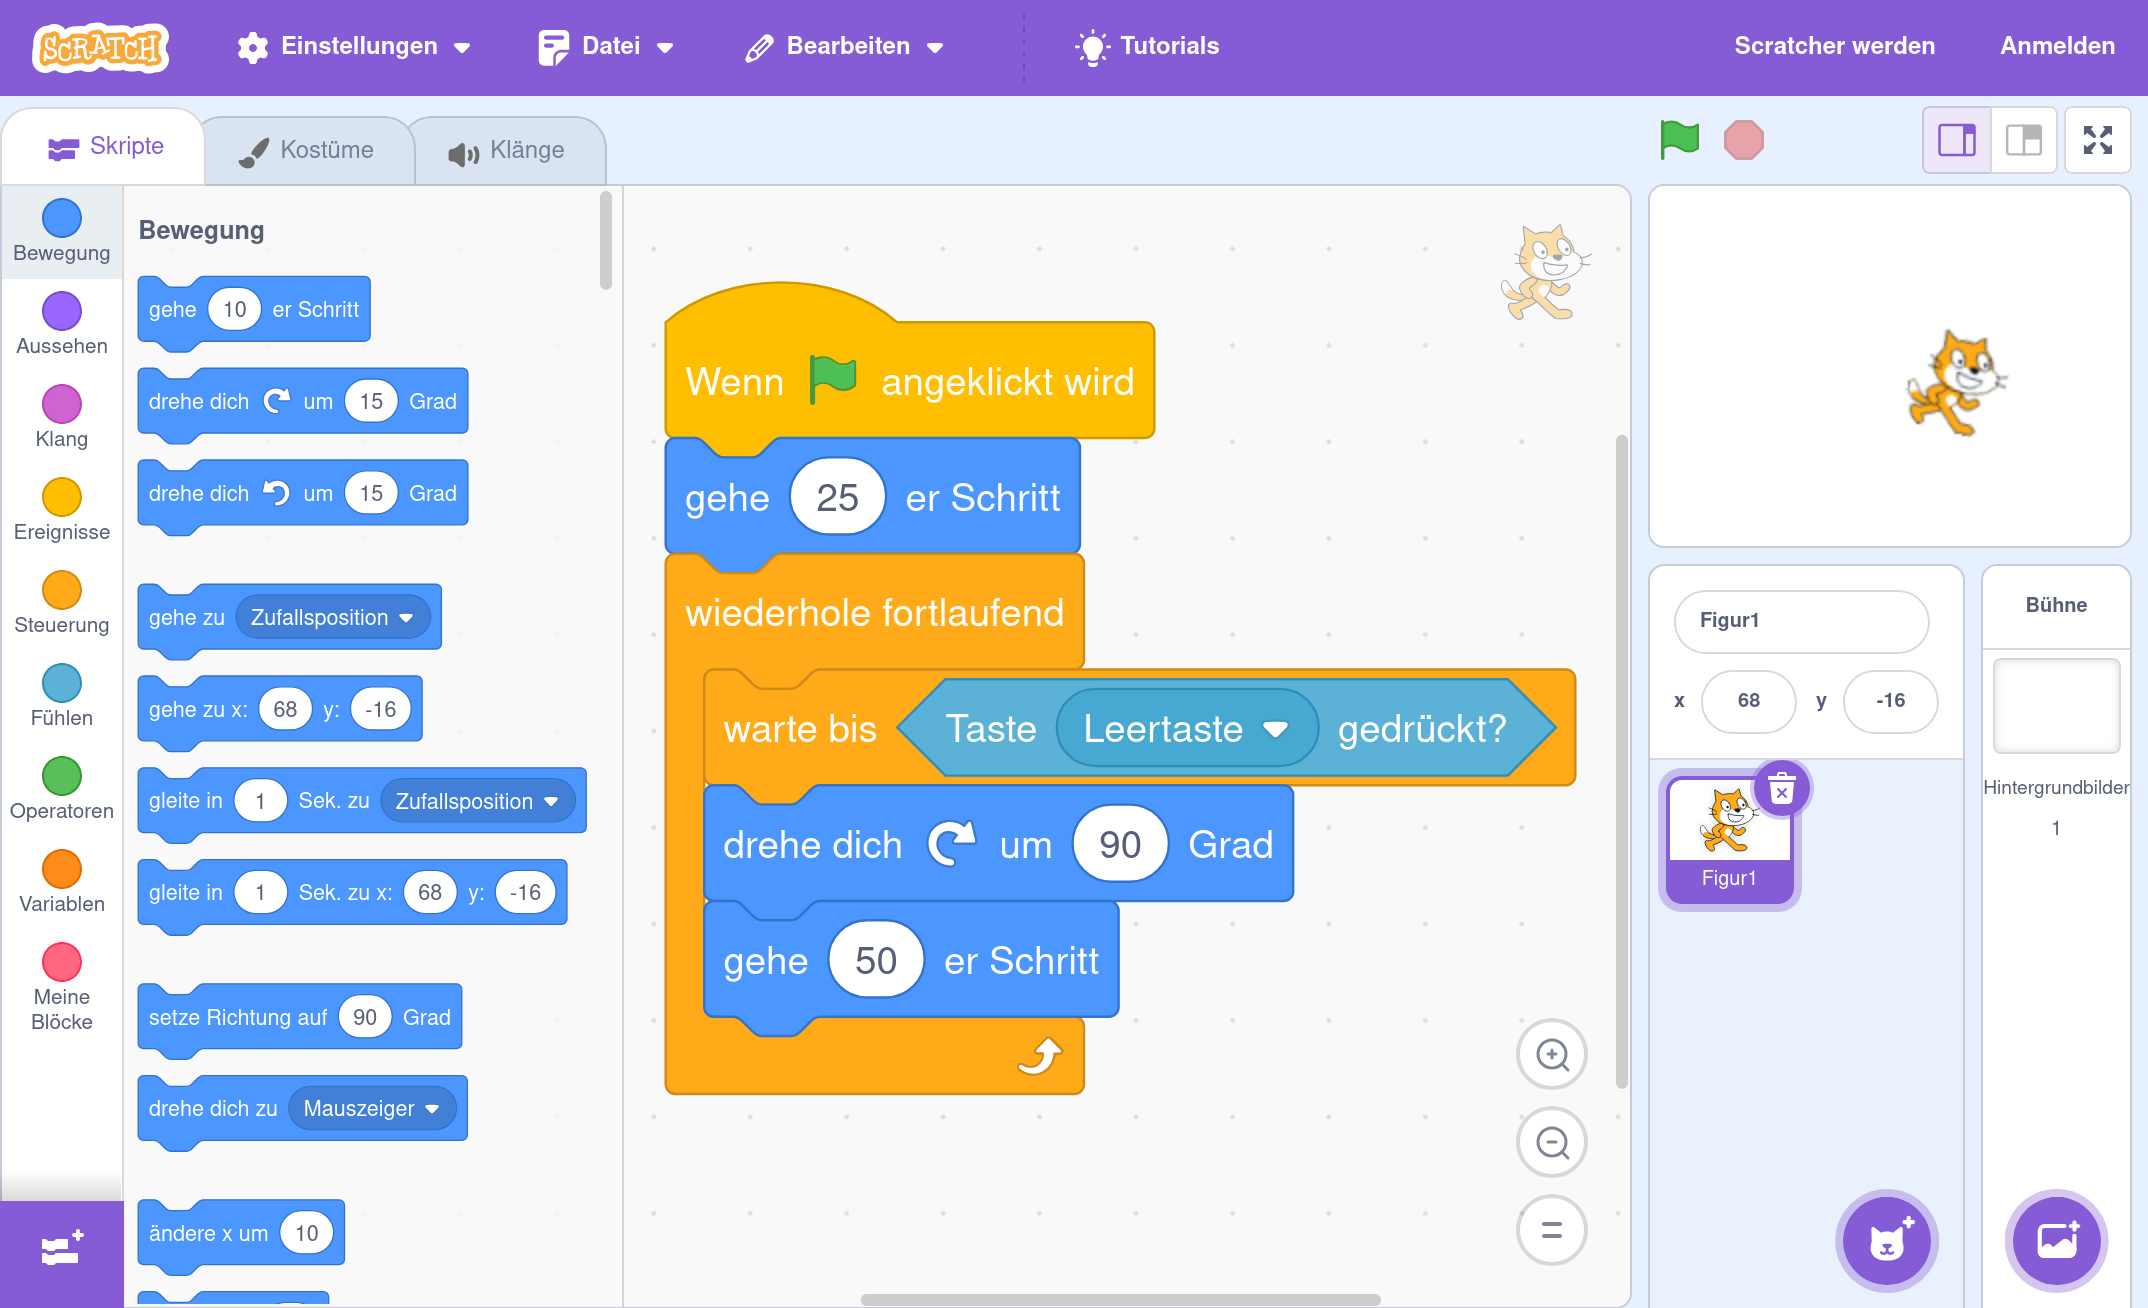
\includegraphics[width=0.95\textwidth]{assets/scratch.png}
  \end{center}
  \caption[Die Programmierumgebung \Scratch{} mit einem Beispielprogramm]{Die Programmierumgebung \Scratch{} mit einem Beispielprogramm. Im linken Bereich können Blöcke ausgewählt werden, die in der Mitte genutzt werden um Skripte zusammenzusetzen. Rechts befindet sich das Ausgabefenster und die Möglichkeit, Figuren und Bühnen zu verwalten.}
  \label{fig:scratch}
\end{figure}

Abbildung \ref{fig:scratch} zeigt den \Scratch{}-Editor und ein Beispielprogramm. Die Ansicht kann in 3 Spalten unterteilt werden. Links können die Blöcke ausgewählt werden, die in der Mitte zusammengesetzt werden sollen. Der rechte Abschnitt ist unterteilt, in einen Ausgabebereich, und ein Verwaltungsbereich für Figuren und Bühnen. Die Blöcke im Auswahlmenü sind thematisch sortiert. Die Farbgebung spiegelt dies wieder (Vgl. Abbildung \ref{fig:scratch-types}). Um Blöcke im Skriptbereich zu verwenden, müssen sie mittels \textit{Drag and Drop} nach rechts gezogen werden. Skripte sind an Figuren gebunden. Im Beispielprogramm wird die Tiger-Figur nach Start des Programms bewegt und rotiert, sobald die Leertaste gedrückt wird.
\parencite{maloneyScratchProgramming2010}

\Scratch{} definiert grundsätzlich vier Blockformen \parencite{maloneyScratchProgramming2010}. In Abbildung \ref{fig:scratch-blocks} werden sie verglichen. \textbf{Befehle} führen Programmlogik aus, die beispielsweise Figuren bewegen oder Variablen anpassen. Sie besitzen typischerweise eine Kerbe am oberen Rand und Verbindungsstelle am unteren Rand. \textbf{Funktionen} geben Werte zurück, die errechnet werden können oder in Variablen gespeichert wurden. Es ist nicht möglich, Funktionen an Blöcke mit Kerben anzufügen, sie können aber in korrespondierende Felder innerhalb von Blöcken eingesetzt werden. \textbf{Auslöser} besitzen keine Kerbe am oberen Rand, und stellen den Anfang der Ausführung des angehängten Konstrukts dar. \textbf{Kontrollstruktur-Blöcke} haben die gleiche Form wie Befehle und können wie sie angewendet werden. Sie beeinflussen den Ablauf des Programms und bilden Programmierkonzepte wie Schleifen und Bedingungen ab. Abbildung \ref{fig:scratch} zeigt eine "wiederhole fortlaufend"-Schleife. Es ist zu sehen, dass diese Art von Block auch weitere Blöcke annehmen kann, die im Schleifenkörper ausgeführt werden \parencite{maloneyScratchProgramming2010}.

\begin{figure}[!ht]
  \begin{center}
    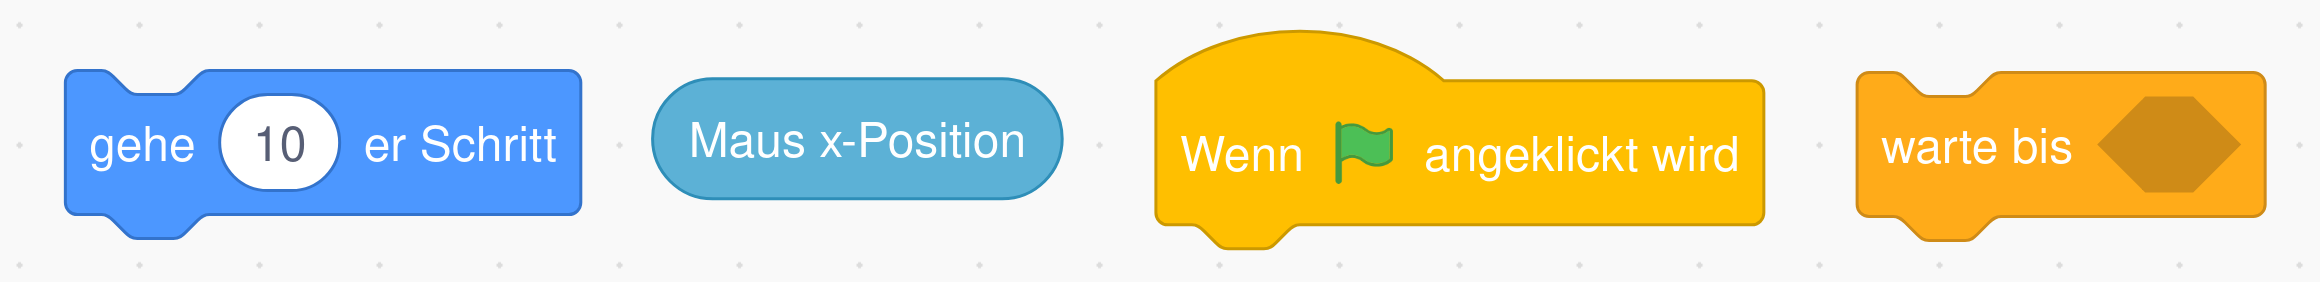
\includegraphics[width=0.95\textwidth]{assets/scratch-blocks.png}
  \end{center}
  \caption[Blockformen in \Scratch{}]{Blockformen in \Scratch{} (v.\,l.\,n.\,r.): Befehl, Funktion, Auslöser, Kontrollstruktur.}
  \label{fig:scratch-blocks}
\end{figure}

Die Programmiersprache \Scratch{} beschränkte sich zunächst auf drei Datentypen \parencite{maloneyScratchProgramming2010}. Dabei handelt es sich um Text, Zahl und Wahrheitswerte. Texte und Zahlen werden als abgerundete Blöcke dargestellt, während Wahrheitswerte sechseckig sind besitzen. In Abbildung \ref{fig:scratch-types} werden zwei Funktionen mit unterschiedlichen Datentypen gezeigt, sowie Blöcke die diese als Eingabewerte entgegennehmen können. In den blauen und lila-farbigen Blöcken können auch manuell Werte eingegeben werden, der blaue Block nimmt jedoch nur Zahlen an. Die Datentypen in \Scratch{} wurden mit Nachfolgeversionen erweitert, Version 1.3 führte beispielsweise Listen ein \parencite{harveyBringingNo2010}.

\begin{figure}[!ht]
  \minipage[t]{.49\textwidth}
  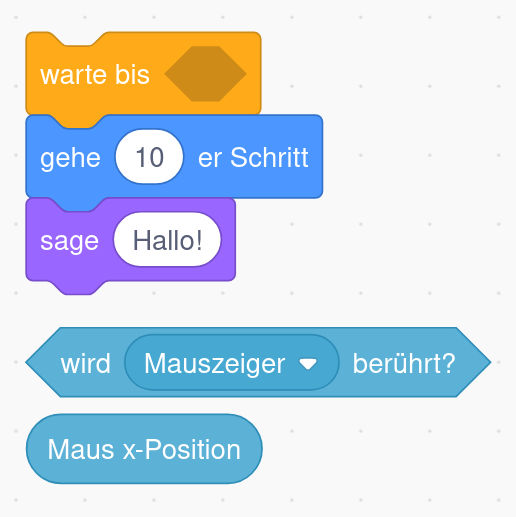
\includegraphics[width=\linewidth]{assets/scratch-types.png}
  \caption[Drei der Blockkategorien in \Scratch{}]{Drei der Blockkategorien in \Scratch{}: Steuerung (Orange), Bewegung (Blau), Aussehen (Lila). Datentypen in \Scratch{}: Boolean (sechseckige Blöcke), Zahlen und Text (abgerundete Blöcke).}
  \label{fig:scratch-types}
  \endminipage
  \hfill
  \minipage[t]{.49\textwidth}
  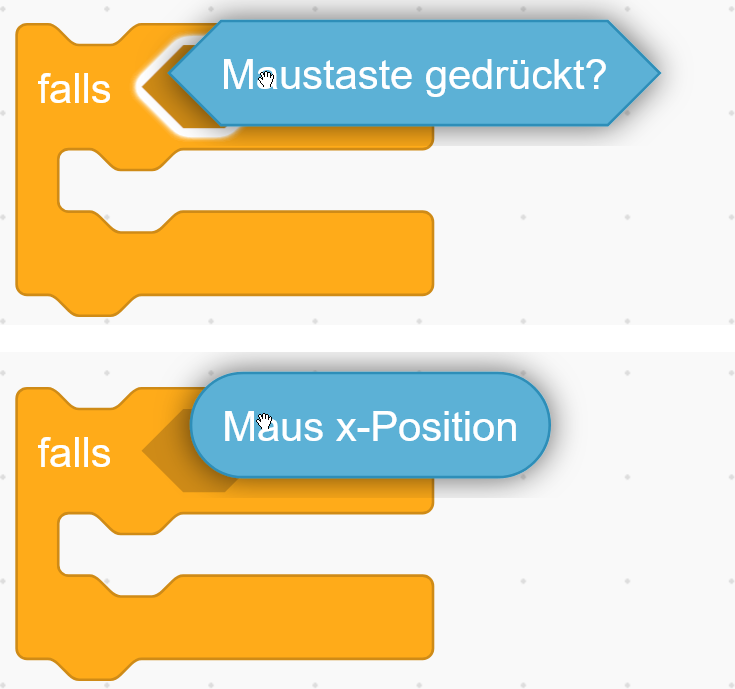
\includegraphics[width=\linewidth]{assets/scratch-drop.png}
  \caption[Indikator beim Zusammensetzen von Blöcken in \Scratch{}]{Blöcke in \Scratch{} können nur ineinander gesetzt werden, wenn der Datentyp übereinstimmt. Dies wird durch einen weißen Indikator vermittelt.}
  \label{fig:scratch-drop}
  \endminipage
\end{figure}

\Scratch{} signalisiert über die Form der Blöcke, ob sie zusammengesetzt werden können. Zusätzlich wird beim \textit{Drag and Drop} über einen weißen Indikator gezeigt, ob Blöcke an der aktuellen Stelle eingesetzt werden können. In Abbildung \ref{fig:scratch-drop} ist zu sehen, wie so signalisiert wird, dass eine Wenn-Abfrage nur Wahrheitswerte annehmen kann.

Eine grundlegende Überlegung die bei der Entwicklung von \Scratch{} getroffen wurde, war das Verzichten auf Fehlermeldungen \parencite{maloneyScratchProgramming2010}. Nutzer:innen sollten anhand der Form der Blöcke erkennen, ob es möglich ist, Elemente miteinander zu kombinieren und durch probieren herausfinden, was funktioniert \parencite{maloneyScratchProgramming2010}.

\Scratch{} wird auch im Bildungsbereich genutzt, sowohl in Schulen \parencite{ortiz-colonTeachingScratch2016}, als auch an Universitäten \parencite{dekerekiScratchApplications2008}. Der Erfolg dieser Anwendung variiert, führt jedoch oft zu Motivationssteigerungen \parencite{dekerekiScratchApplications2008, martinez-valdesRelativelyUnsatisfactory2017}. Dies ist besonders bei jüngeren Zielgruppen der Fall \parencite{ortiz-colonTeachingScratch2016}.

\subsubsection{Snap!}
\Snap{} stellt eine Neuimplementierung von \Scratch{} mit neuen Funktionen dar. \textcite{harveyBringingNo2010} stellte in zeitigen Versionen von \Scratch{} Einschränkungen fest, die es für die Benutzung zur Lehre in der höheren Bildung ungeeignet macht. Einerseits gab es keine Funktionen, wodurch keine Rekursion abgebildet werden konnte, andererseits wurden komplexe Datenstrukturen nicht unterstützt \parencite{harveyBringingNo2010}.

\begin{figure}[!ht]
  \minipage[t]{.575\textwidth}
  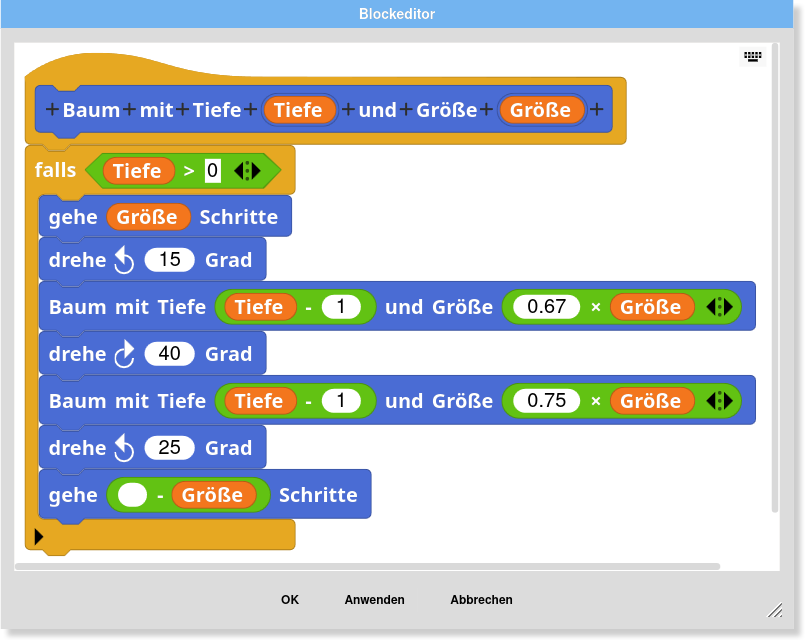
\includegraphics[width=\linewidth]{assets/snap-edit.png}
  \caption[Definition einer rekursiven Funktion in \Snap{}]{Definition einer rekursiven Funktion in \Snap{}, am Beispiel von \textcite{harveyBringingNo2010}. Die Definition bewegt die Figur entlang eines Pfades, der die Form eines binären Baums mit der spezifizierten Tiefe und Größe besitzt.}
  \label{fig:snap-edit}
  \endminipage
  \hfill
  \begin{minipage}[t]{.405\textwidth}
    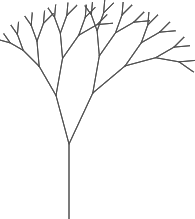
\includegraphics[width=\linewidth]{assets/snap-tree.png}
    \caption[Ergebnis der Funktion aus Abbildung \ref*{fig:snap-edit}]{Ergebnis der Funktion aus Abbildung \ref{fig:snap-edit}. Vor dem Funktionsaufruf wurde das Zeichnen des Pfades angeschaltet.}
    \label{fig:snap-tree}
  \end{minipage}
\end{figure}

Um Rekursion in \Scratch{} umzusetzten, wurde eine Erweiterung namens \ac{BYOB} entwickelt, die es Nutzer:innen erlaubt, eigene Blöcke zu definieren \parencite{harveyBringingNo2010}. Später wurde diese Erweiterung zu einer eigenständigen Anwendung, \Snap{}, welche diese und weitere Funktionalitäten enthält. Abbildungen \ref{fig:snap-edit} und \ref{fig:snap-tree} zeigen die Definition und das Ergebnis einer rekursiven Funktion, die als Block definiert wurde, und sich somit selbst aufrufen kann.

\Snap{} verallgemeinert die Datentypen von \Scratch{} und ermöglicht somit tiefgreifenderen Zugriff auf Variablen. So ist es zum Beispiel möglich, über den Listen-Block Listen zu erstellen, die nicht zuvor als Variable definiert werden müssen. Das ermöglicht Listen in Listen und komplexere Datentypen \parencite{harveySnapReference2020}.

\begin{figure}
  \centering
  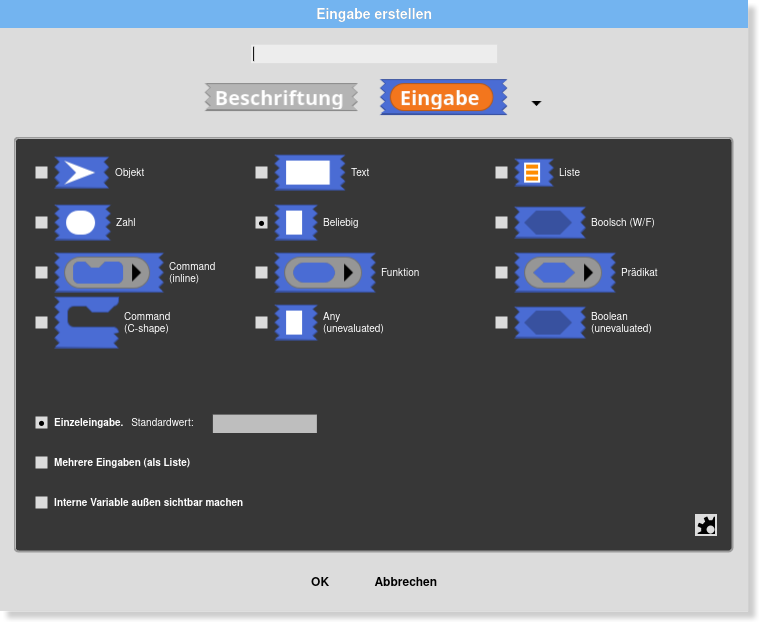
\includegraphics[width=0.57\textwidth]{assets/snap-input-types.png}
  \caption[Dialog zur Definition eines Parameters in \Snap{}]{Ausführlicher Dialog zur Definition eines Parameters in \Snap{}. Die Auswahlmöglichkeiten kontrollieren das spätere Verhalten des Blocks.}
  \label{fig:snap-input-types}
\end{figure}

Außerdem unterstützt \Snap{} Ansätze der funktionalen Programmierung, indem Funktionen als Daten übergeben werden können. Ein Beispiel dafür stellt der "Wende ... an auf ...", welches eine Funktion im ersten Parameter entgegennimmt und auf alle Elemente der Liste im zweiten Parameter anwendet \parencite{harveySnapReference2020}. Diese Möglichkeit, gekoppelt mit Blöcken zum Klonen von Figuren und Funktionen, ermöglicht wiederum objektorientierte Programmierung innerhalb von \Snap{} \parencite{harveySnapReference2020}. Figuren werden in \Snap{} auch als Objekte bezeichnet.

Wie in Abbildung \ref{fig:snap-input-types} zu sehen, unterstützt der Editor für Eingabeparameter von Blöcken unterschiedliche Parametertypen. Somit können während der Erstellung eines Blocks die Einstellungen so gewählt werden, dass die Bedienung des Blocks erleichtert wird. \Snap{} kennt die Eingabetypen des Blocks und kann somit sicherstellen, dass nur passende Blöcke in die Eingabefelder eingesetzt werden \parencite{harveySnapReference2020}. Des Weiteren ist es möglich Dropdown-Menüs zur Auswahl bestimmter Werte für ein Eingabefeld zu definieren. \Snap{} erweitert den in Abbildung \ref{fig:scratch-drop} gezeigten Ansatz, indem beim \textit{Drag and Drop} ein roter Indikator angezeigt wird, wenn der Typ nicht übereinstimmt \parencite{harveySnapReference2020}.

Während das Aussehen der \Snap{}-Programmierumgebung \Scratch{} stark ähnelt, wurde \Snap{} mit einigen Funktionalitäten angereichert, die dazu führen, dass komplexe Konzepte der Programmierung in einem blockbasierten Editor erlernt werden können \parencite{ballSnapLook2019}. Eingesetzt wird es beispielsweise im Kurs \textit{"The Beauty and Joy of Computing"} der \citeauthor{universityofcaliforniaberkeleyBeautyJoy}, welcher sich an Studiengänge außerhalb der Informatik richtet \parencite{universityofcaliforniaberkeleyBeautyJoy}.

\subsubsection{DataSnap}
\citeauthor{hellmannDataSnapEnabling2015} präsentiert in seiner Master-Arbeit eine Erweiterung zu \Snap{}, die sich an Fachexpert:innen richtet. Ziel dieser Arbeit war es, Nutzer:innen zu erlauben, die blockbasierte Oberfläche von \Snap{} zu nutzen um mehrere Schritte der Datenverarbeitung zu absolvieren. Die folgenden Ziele wurden dabei definiert \parencite{hellmannDataSnapEnabling2015}:

\begin{itemize}
  \item Einfaches Importieren von Daten.
  \item Benutzung von \Snap{}-Blöcken zur Definition der Datenverarbeitung.
  \item Nutzung von externen Rechnern zur Beschleunigung der Auswertung.
  \item Visualisierung der Ergebnisse.
\end{itemize}

\DataSnap{} stellt eine Erweiterung dar, die genannten Ziele in \Snap{} ermöglicht. Mit der Erweiterung können Daten auf dem Server importiert werden, die dann auf Basis einer mit Blöcken definierten Vorschrift ausgewertet werden können. Auch dies kann auf dem Server passieren. Die resultierenden Daten werden dann an den Browser zurückgeschickt und können dort visualisiert werden \parencite{hellmannDataSnapEnabling2015}.

Da \Snap{} keine Möglichkeit zum Importieren von großen Datensätzen bietet, führt \DataSnap{} Blöcke zum Import von Daten an. Die Implementation beschränkt sich auf den Import von \acs{CSV}-Dateien, welche unter einer URL erreichbar sind. Da es sich um potentiell große Datensätze handelt, werden diese Daten nicht im Browser der Anwender:innen gespeichert, sondern auf einem Server \parencite{hellmannDataSnapEnabling2015}. Für den Zugriff auf die sogenannten \textit{"cloud variables"} wurde eigens Blöcke erstellt, die sich von den Blöcken für lokale Variablen unterscheiden \parencite{hellmannDataSnapEnabling2015}.

\begin{figure}[!ht]
  \begin{minipage}[t]{.52\textwidth}
    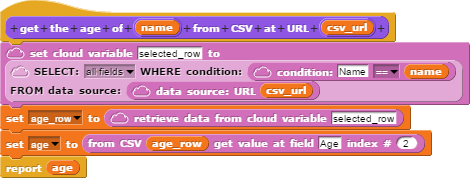
\includegraphics[width=\linewidth]{assets/datasnap-method-edit.png}
    \caption[Definition eines Blocks in \DataSnap{}]{Definition für einen Block in \DataSnap{}, welcher das Alter einer Person aus einer \acs{CSV}-Datei aussucht, deren Spalten \texttt{Name} und \texttt{Age} sind.}
    \label{fig:datasnap-method-edit}
  \end{minipage}
  \hfill
  \begin{minipage}[t]{.46\textwidth}
    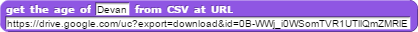
\includegraphics[width=\linewidth]{assets/datasnap-method-use.png}
    \caption[Benutzung der in Abbildung \ref*{fig:datasnap-method-edit} definierten Funktion]{Benutzung der in \ref{fig:datasnap-method-edit} definierten Funktion. Als Parameter werden ein Name und die \acs{URL} einer \acs{CSV}-Datei angegeben.}
    \label{fig:datasnap-method-use}
  \end{minipage}
\end{figure}

Zur Verarbeitung der Daten können die nativen \Snap{}-Blöcke nur begrenzt verwendet werden. Zur Unterstützung von tabellarischen CSV-Datenstrukturen wurden eigens Blöcke definiert, die \acs{SQL}-Abfragen ähneln und auf dem Server ausgewertet werden \parencite{hellmannDataSnapEnabling2015}. Abbildung \ref{fig:datasnap-method-edit} zeigt die Nutzung solcher \textit{"cloud methods"}, um eine wiederverwendbare Abfrage als Block zu definieren. Die von \DataSnap{} hinzugefügten Blöcke werden rosa und pink dargestellt. Im Beispiel werden die Daten von einer \acs{CSV}-Datei abgerufen, die bei der Verwendung des Blocks (Abbildung \ref{fig:datasnap-method-use}) angegeben wird.

Außerdem definiert \DataSnap{} Blöcke zur Visualisierung von Datensätzen in \Snap{} \parencite{hellmannDataSnapEnabling2015}. Abbildung \ref{fig:datasnap-visualization} zeigt, wie dies mit Daten mit geographischem Bezug stattfinden kann. Das Beispiel nutzt Blöcke, um den Ort und die Größenordnung von Erdbeben in Nordamerika auf einer Karte zu markieren.

\begin{figure}[!ht]
  \centering
  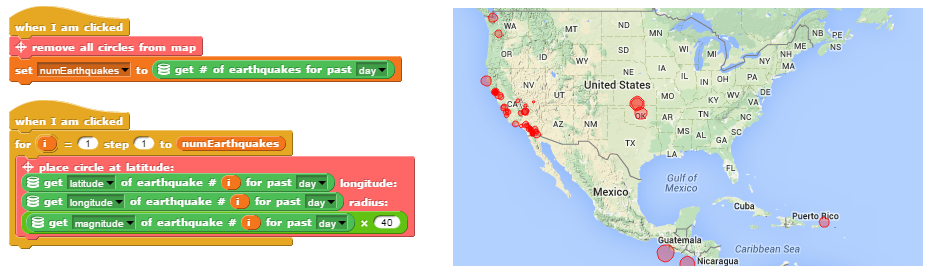
\includegraphics[width=0.95\textwidth]{assets/datasnap-visualization.png}
  \caption[Visualisierung eines Datensatzes über Erdbeben in \Snap{}]{Visualisierung eines Datensatzes über Erdbeben in \DataSnap{}. Es wird eine Schleife benutzt, um alle Erdbeben auszuwählen, und sie mit einem Kreis an ihrem Ursprungsort zu markieren. Der Radius der Kreise entspricht der Größenordnung der Erdbeben.\\\parencite[28]{hellmannDataSnapEnabling2015}}
  \label{fig:datasnap-visualization}
\end{figure}

Es kann festgehalten werden, dass \Snap{} durch die Erweiterung \DataSnap{} zu einem Werkzeug wird, welches auch zur Auswertung von Daten durch Fachanwender:innen benutzt werden kann \parencite{hellmannDataSnapEnabling2015}. Somit richtet es sich an eine ähnliche Zielgruppe wie der in dieser Arbeit entwickelte Block-Editor. Der Block-Editor befasst sich jedoch nicht mit dem Import der Daten, da dies bereits aus verschiedenen Datenformaten in Simplex4TwIS stattfindet (Vgl. \ref{sec:simplex-importer}). Die Visualisierungskomponente entfällt ebenso und wird in Simplex4TwIS über andere Teilsystem oder durch externe Programme durchgeführt.
